\documentclass[10pt]{article}
\usepackage{graphicx}
\usepackage{mathtools}
\usepackage{listings}

\begin{document}
	\section*{Questions 7}
	\begin{enumerate}
		\item How do you allocate GSL vectors and matrices?
		
		To allocate a GSL vectors, you type:

		\texttt{gsl\_vector *v1 = gsl\_vector\_alloc (size\_t n);}

		\texttt{gsl\_vector *v2 = gsl\_vector\_calloc (size\_t n);}

		To allocate a GSL matrix, you type:

		\texttt{gsl\_matrix *m1 = gsl\_vector\_alloc (size\_t n1, size\_t n2);}

		\texttt{gsl\_matrix *m2 = gsl\_vector\_calloc (size\_t n1, size\_t n2);}

		the difference between \texttt{alloc} and \texttt{calloc}, is that \texttt{calloc} initializes all the elements as zeros, where \texttt{alloc} doesn't.
		In the end, you will need to free them, with

		\texttt{gsl\_vector\_free (gsl\_vector *v);}

		\texttt{gsl\_matrix\_free (gsl\_vector *m);}
		
	\end{enumerate}
	\section*{Problem 20: Implement the Arctangent function using integral representation.}
	\begin{align}
		\mathrm{arctan}(x) 
		= \int_{0}^{x} \frac{1}{z^2+1} \, dz. \label{eq:integration_func}
	\end{align}
	To facilitate numerical integration reduce the argument to a reasonable interval (e.g. $[0,1]$) using the formulae (check them),
	\begin{align}
		\mathrm{arctan}(-x) = -\mathrm{arctan}(x) \\
		\mathrm{arctan}\!\left(\frac{1}{x}\right) =
		\frac{\pi}{2} - \mathrm{arctan}(x), \ \text{ if } x > 0.
	\end{align}
	prior to integration. Compare with the corresponding function from \texttt{<math.h>} or from \texttt{GSL}.
	
	The problem was solved by integrating with \texttt{gsl/gsl\_integratson.h}. First the integrand from eq.~\ref{eq:integration_func} was define:
	\lstinputlisting[language=C, firstline=6, lastline=8]{my_math.c}
	 and then the GSL integration rutine was build:
	\lstinputlisting[language=C, firstline=10]{my_math.c}
	The three if statements ensures that the function only integrates in the range of $[0,1]$.
	
	The result of the integration was compared using \texttt{atan(x)} from \texttt{<math.h>} in the main function, and plottet with points, see fig.~\ref{fig:arctan_plot}.

	\begin{figure}[hb]
	\centering
	% GNUPLOT: LaTeX picture with Postscript
\begingroup
  \makeatletter
  \providecommand\color[2][]{%
    \GenericError{(gnuplot) \space\space\space\@spaces}{%
      Package color not loaded in conjunction with
      terminal option `colourtext'%
    }{See the gnuplot documentation for explanation.%
    }{Either use 'blacktext' in gnuplot or load the package
      color.sty in LaTeX.}%
    \renewcommand\color[2][]{}%
  }%
  \providecommand\includegraphics[2][]{%
    \GenericError{(gnuplot) \space\space\space\@spaces}{%
      Package graphicx or graphics not loaded%
    }{See the gnuplot documentation for explanation.%
    }{The gnuplot epslatex terminal needs graphicx.sty or graphics.sty.}%
    \renewcommand\includegraphics[2][]{}%
  }%
  \providecommand\rotatebox[2]{#2}%
  \@ifundefined{ifGPcolor}{%
    \newif\ifGPcolor
    \GPcolortrue
  }{}%
  \@ifundefined{ifGPblacktext}{%
    \newif\ifGPblacktext
    \GPblacktexttrue
  }{}%
  % define a \g@addto@macro without @ in the name:
  \let\gplgaddtomacro\g@addto@macro
  % define empty templates for all commands taking text:
  \gdef\gplbacktext{}%
  \gdef\gplfronttext{}%
  \makeatother
  \ifGPblacktext
    % no textcolor at all
    \def\colorrgb#1{}%
    \def\colorgray#1{}%
  \else
    % gray or color?
    \ifGPcolor
      \def\colorrgb#1{\color[rgb]{#1}}%
      \def\colorgray#1{\color[gray]{#1}}%
      \expandafter\def\csname LTw\endcsname{\color{white}}%
      \expandafter\def\csname LTb\endcsname{\color{black}}%
      \expandafter\def\csname LTa\endcsname{\color{black}}%
      \expandafter\def\csname LT0\endcsname{\color[rgb]{1,0,0}}%
      \expandafter\def\csname LT1\endcsname{\color[rgb]{0,1,0}}%
      \expandafter\def\csname LT2\endcsname{\color[rgb]{0,0,1}}%
      \expandafter\def\csname LT3\endcsname{\color[rgb]{1,0,1}}%
      \expandafter\def\csname LT4\endcsname{\color[rgb]{0,1,1}}%
      \expandafter\def\csname LT5\endcsname{\color[rgb]{1,1,0}}%
      \expandafter\def\csname LT6\endcsname{\color[rgb]{0,0,0}}%
      \expandafter\def\csname LT7\endcsname{\color[rgb]{1,0.3,0}}%
      \expandafter\def\csname LT8\endcsname{\color[rgb]{0.5,0.5,0.5}}%
    \else
      % gray
      \def\colorrgb#1{\color{black}}%
      \def\colorgray#1{\color[gray]{#1}}%
      \expandafter\def\csname LTw\endcsname{\color{white}}%
      \expandafter\def\csname LTb\endcsname{\color{black}}%
      \expandafter\def\csname LTa\endcsname{\color{black}}%
      \expandafter\def\csname LT0\endcsname{\color{black}}%
      \expandafter\def\csname LT1\endcsname{\color{black}}%
      \expandafter\def\csname LT2\endcsname{\color{black}}%
      \expandafter\def\csname LT3\endcsname{\color{black}}%
      \expandafter\def\csname LT4\endcsname{\color{black}}%
      \expandafter\def\csname LT5\endcsname{\color{black}}%
      \expandafter\def\csname LT6\endcsname{\color{black}}%
      \expandafter\def\csname LT7\endcsname{\color{black}}%
      \expandafter\def\csname LT8\endcsname{\color{black}}%
    \fi
  \fi
    \setlength{\unitlength}{0.0500bp}%
    \ifx\gptboxheight\undefined%
      \newlength{\gptboxheight}%
      \newlength{\gptboxwidth}%
      \newsavebox{\gptboxtext}%
    \fi%
    \setlength{\fboxrule}{0.5pt}%
    \setlength{\fboxsep}{1pt}%
\begin{picture}(7200.00,5040.00)%
    \gplgaddtomacro\gplbacktext{%
      \csname LTb\endcsname%
      \put(814,704){\makebox(0,0)[r]{\strut{}$0.5$}}%
      \put(814,1518){\makebox(0,0)[r]{\strut{}$1$}}%
      \put(814,2332){\makebox(0,0)[r]{\strut{}$1.5$}}%
      \put(814,3147){\makebox(0,0)[r]{\strut{}$2$}}%
      \put(814,3961){\makebox(0,0)[r]{\strut{}$2.5$}}%
      \put(814,4775){\makebox(0,0)[r]{\strut{}$3$}}%
      \put(946,484){\makebox(0,0){\strut{}$0$}}%
      \put(1532,484){\makebox(0,0){\strut{}$1$}}%
      \put(2117,484){\makebox(0,0){\strut{}$2$}}%
      \put(2703,484){\makebox(0,0){\strut{}$3$}}%
      \put(3289,484){\makebox(0,0){\strut{}$4$}}%
      \put(3875,484){\makebox(0,0){\strut{}$5$}}%
      \put(4460,484){\makebox(0,0){\strut{}$6$}}%
      \put(5046,484){\makebox(0,0){\strut{}$7$}}%
      \put(5632,484){\makebox(0,0){\strut{}$8$}}%
      \put(6217,484){\makebox(0,0){\strut{}$9$}}%
      \put(6803,484){\makebox(0,0){\strut{}$10$}}%
    }%
    \gplgaddtomacro\gplfronttext{%
      \csname LTb\endcsname%
      \put(176,2739){\rotatebox{-270}{\makebox(0,0){\strut{}$\mathrm E(\alpha)$}}}%
      \put(3874,154){\makebox(0,0){\strut{}$\alpha$}}%
      \csname LTb\endcsname%
      \put(5816,4272){\makebox(0,0)[r]{\strut{}$\mathrm E(\alpha) \equiv \frac{\langle \Psi_{\alpha} \mid \mathrm{H}_{os} \mid \Psi_{\alpha} \rangle}{\langle \Psi_{\alpha} \mid \Psi_{\alpha} \rangle}$}}%
    }%
    \gplbacktext
    \put(0,0){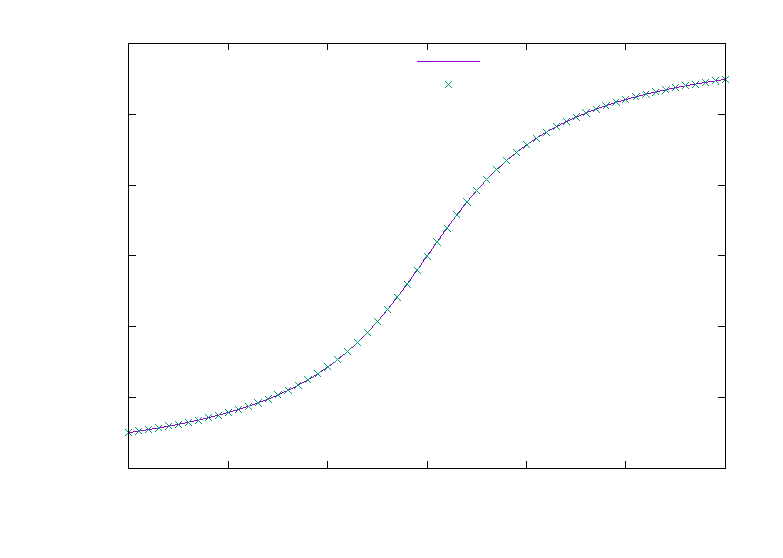
\includegraphics{plot}}%
    \gplfronttext
  \end{picture}%
\endgroup

	\caption{Plot of calculated and exact arctan(x), every 10th result of the arctan from math.h was plottet as points for clarity.}
	\label{fig:arctan_plot}
	\end{figure}
\end{document}
